\documentclass{report}
\usepackage{polski}
\usepackage[utf8]{inputenc}
\usepackage{float}
\usepackage{graphicx}
\usepackage{caption}
\usepackage{subcaption}
\usepackage{ragged2e}
\usepackage{amsmath}
\usepackage{blindtext}
\usepackage{hyperref}
\begin{document}
\author{Jakub Ogrodowczyk}

\section*{Zadanie 1}
\subsection*{Opis algorytmu}
Korzystamy tutaj z algorytmu Edmondsa-Karpa. Jest to wariacja
algorytmu Forda-Fulkersona, która do wyznaczania ścieżek
używa BFS. Dzięki temu osiągamy złożoność $O(VE^2)$.
\subsection*{Wykresy algorytmu Edmondsa-Karpa}
\begin{figure}[H]
    \centering
    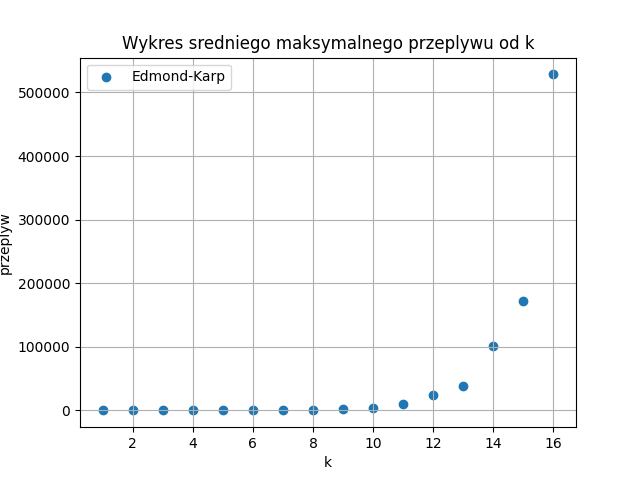
\includegraphics[scale=0.55]{../ex1_and_4/plots/karp_maxflow.png}
    \caption{Średni maksymalny przepływ w zależności od k}
\end{figure}
\begin{figure}[H]
    \centering
    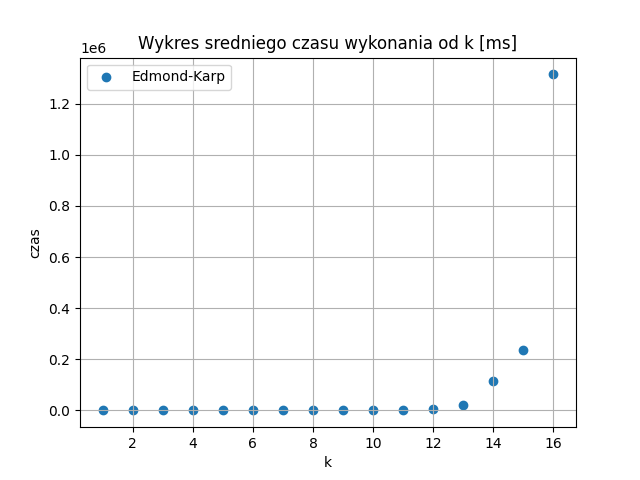
\includegraphics[scale=0.55]{../ex1_and_4/plots/karp_time.png}
    \caption{Średni czas wykonania w zależności od k}
\end{figure}
\begin{figure}[H]
    \centering
    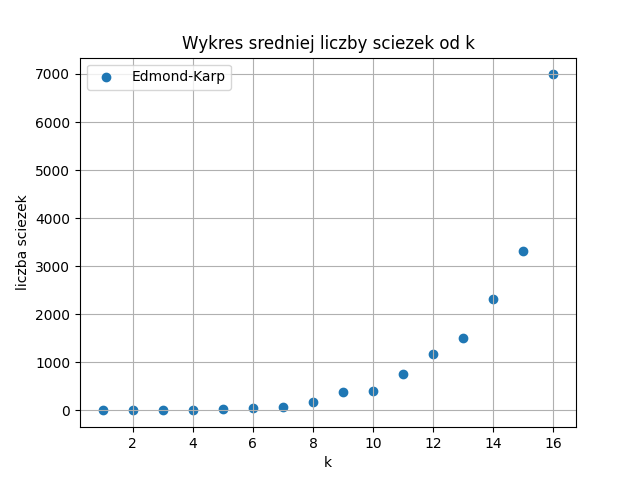
\includegraphics[scale=0.55]{../ex1_and_4/plots/karp_paths.png}
    \caption{Średnia ilość ścieżek w zależności od k}
\end{figure}

\section*{Zadanie 2}
\subsection*{Wykresy}
\begin{figure}[H]
    \centering
    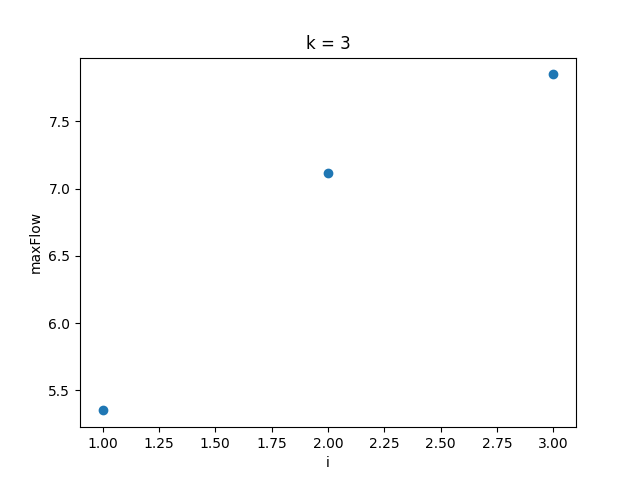
\includegraphics[scale=0.55]{../ex2/plots/k3.png}
    \caption{Maksymalne skojarzenie w zależności od i}
\end{figure}
\begin{figure}[H]
    \centering
    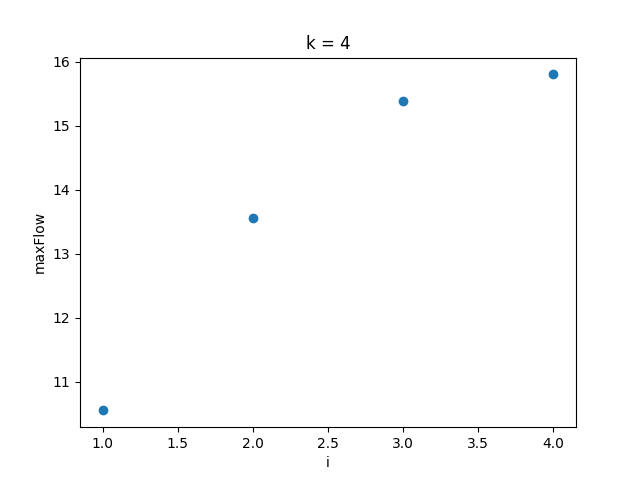
\includegraphics[scale=0.55]{../ex2/plots/k4.png}
    \caption{Maksymalne skojarzenie w zależności od i}
\end{figure}
\begin{figure}[H]
    \centering
    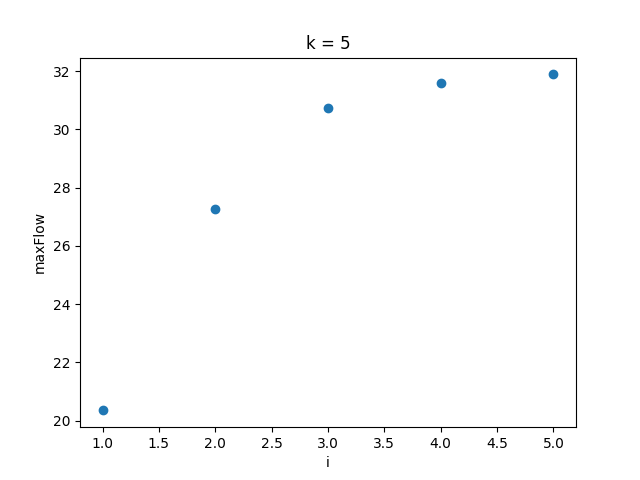
\includegraphics[scale=0.55]{../ex2/plots/k5.png}
    \caption{Maksymalne skojarzenie w zależności od i}
\end{figure}
\begin{figure}[H]
    \centering
    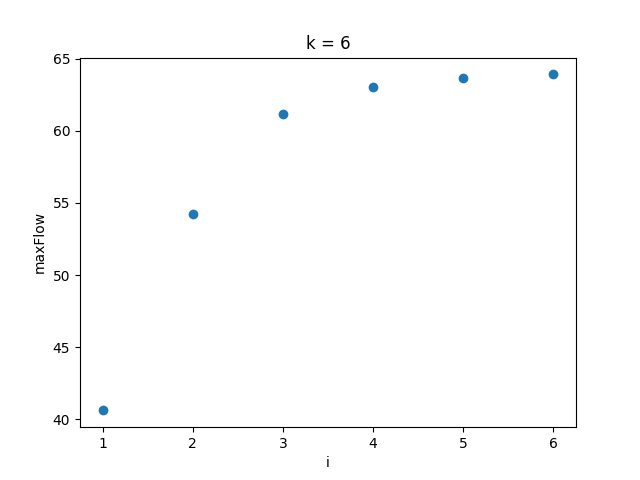
\includegraphics[scale=0.55]{../ex2/plots/k6.png}
    \caption{Maksymalne skojarzenie w zależności od i}
\end{figure}
\begin{figure}[H]
    \centering
    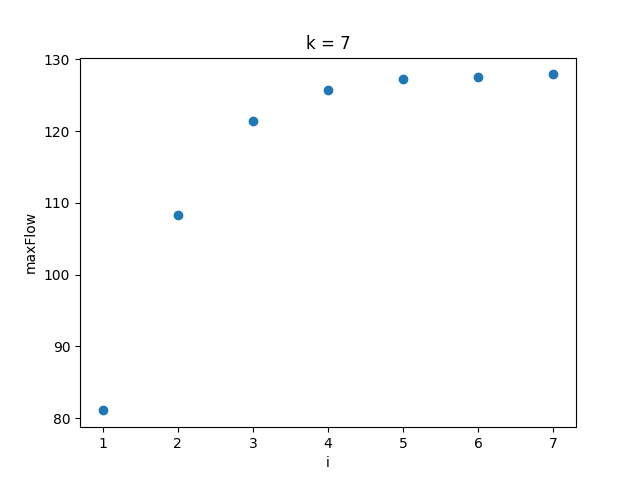
\includegraphics[scale=0.55]{../ex2/plots/k7.png}
    \caption{Maksymalne skojarzenie w zależności od i}
\end{figure}
\begin{figure}[H]
    \centering
    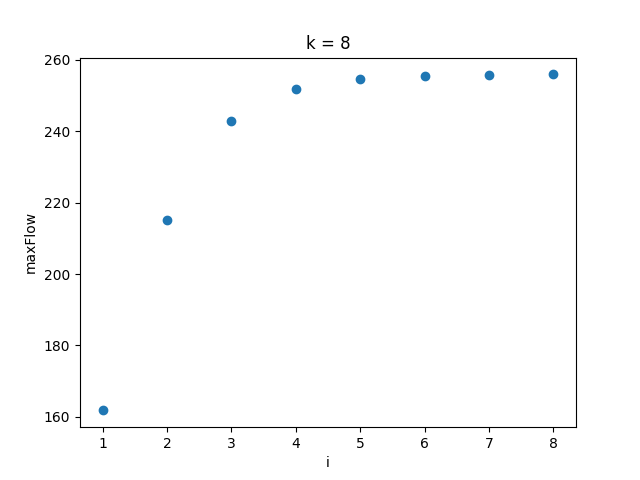
\includegraphics[scale=0.55]{../ex2/plots/k8.png}
    \caption{Maksymalne skojarzenie w zależności od i}
\end{figure}
\begin{figure}[H]
    \centering
    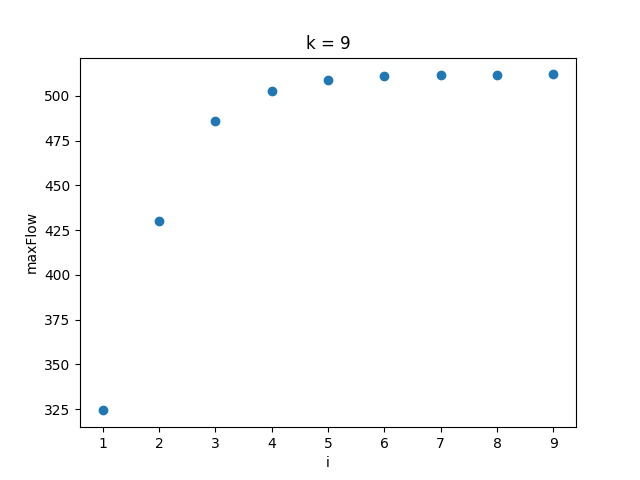
\includegraphics[scale=0.55]{../ex2/plots/k9.png}
    \caption{Maksymalne skojarzenie w zależności od i}
\end{figure}
\begin{figure}[H]
    \centering
    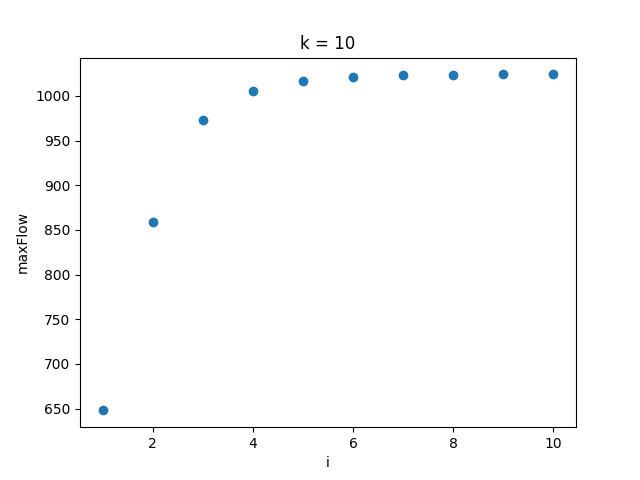
\includegraphics[scale=0.55]{../ex2/plots/k10.png}
    \caption{Maksymalne skojarzenie w zależności od i}
\end{figure}

\section*{Zadanie 4}
\subsection*{Opis algorytmu}
W tym zadaniu korzystam z algorytmu Dinica. Polega on na tym,
że zamiast wysyłać pojedyncze przepływy, wysyłamy wiele naraz
na podstawie grafu poziomów, tj. odległości od celu, który otrzymujemy
przy pomocy zmodyfikowanego BFS'a. Złożoność tego algorytmu to
$O(EV^2)$, co oczywiście jest znacznym przyspieszeniem dla naszej hiperkostki,
gdzie $|V| = 2^k$, a $|E| = k2^{k-1}$.
\subsection*{Wykresy algorytmu Dinica}
\begin{figure}[H]
    \centering
    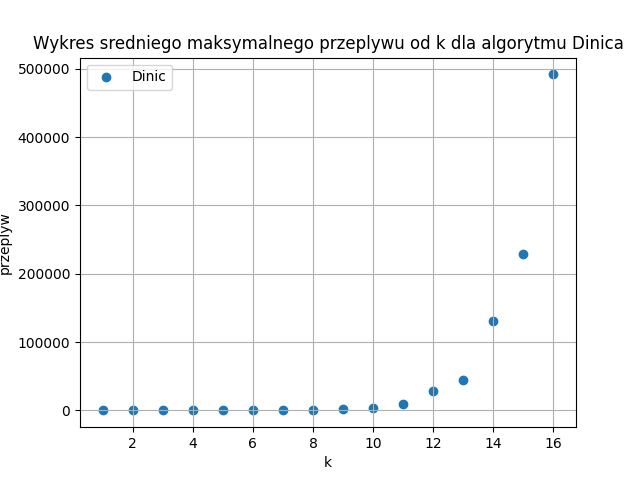
\includegraphics[scale=0.55]{../ex1_and_4/plots/dinic_maxflow.png}
    \caption{Średni maksymalny przepływ w zależności od k}
\end{figure}
\begin{figure}[H]
    \centering
    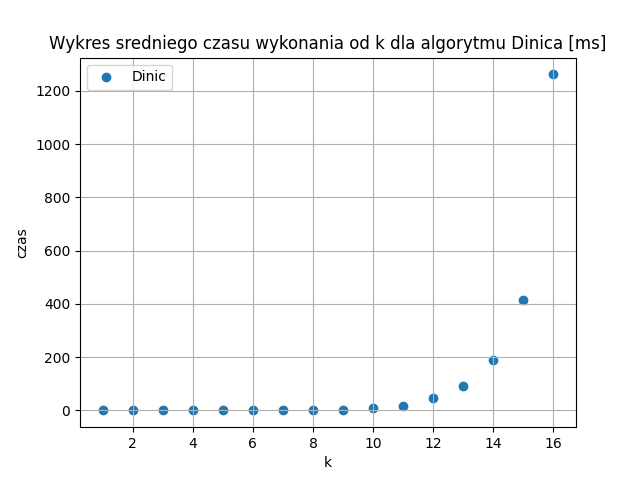
\includegraphics[scale=0.55]{../ex1_and_4/plots/dinic_time.png}
    \caption{Średni czas wykonania w zależności od k}
\end{figure}
\begin{figure}[H]
    \centering
    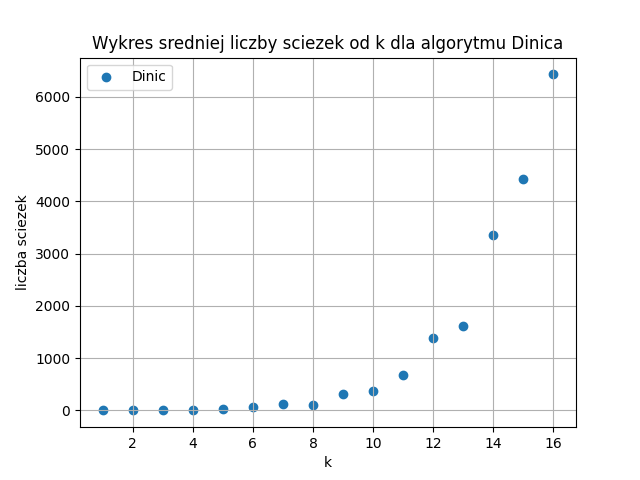
\includegraphics[scale=0.55]{../ex1_and_4/plots/dinic_paths.png}
    \caption{Średnia ilość ścieżek w zależności od k}
\end{figure}
\subsection*{Porównanie Dinica i Edmondsa-Karpa}
\begin{figure}[H]
    \centering
    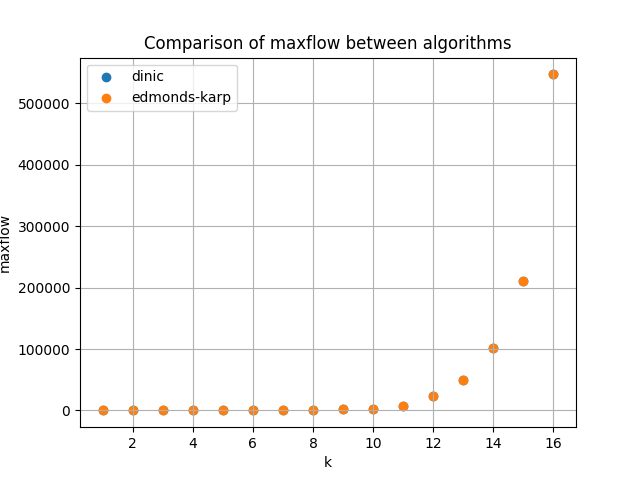
\includegraphics[scale=0.55]{../ex1_and_4/plots/karp_vs_dinic_maxflow.png}
    \caption{Średni maksymalny przepływ w zależności od k}
\end{figure}
\begin{figure}[H]
    \centering
    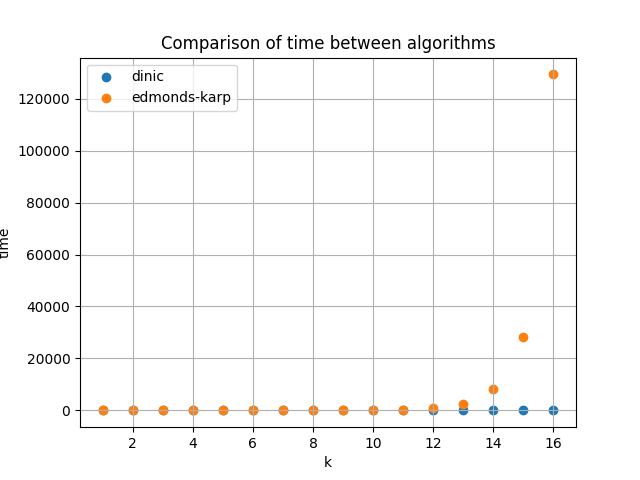
\includegraphics[scale=0.55]{../ex1_and_4/plots/karp_vs_dinic_time.png}
    \caption{Średni czas wykonania w zależności od k}
\end{figure}
\begin{figure}[H]
    \centering
    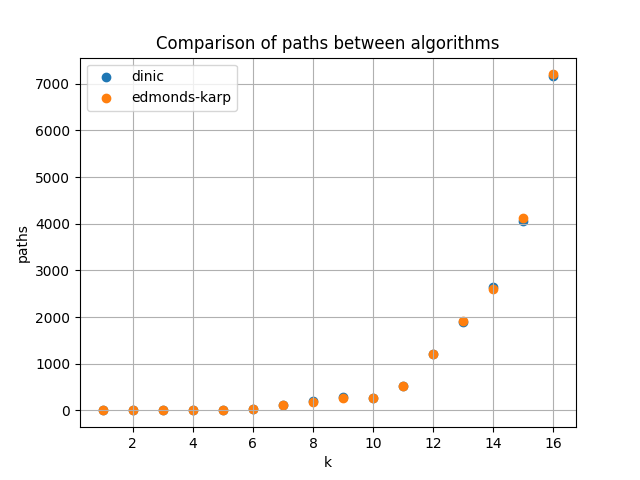
\includegraphics[scale=0.55]{../ex1_and_4/plots/karp_vs_dinic_paths.png}
    \caption{Średnia ilość ścieżek w zależności od k}
\end{figure}

\subsection*{Wnioski}
Zgodnie z oczekiwaniami, algorytm Dinica jest znacznie
wydajniejszy w przypadku naszego grafu ze względu na złożoność,
$O(EV^2)$ vs $O(VE^2)$, gdzie oczywiście nasza kostka ma znacznie
więcej krawędzi niż wierzchołków dla $k > 2$.

\end{document}